\documentclass{beamer}
\usetheme{Madrid}
\usecolortheme{seahorse}
\usepackage{graphicx}
\usepackage{booktabs}
\title[Navier--Stokes Solvers]{High-Order Navier--Stokes Solvers\\Finite Difference and Fourier Spectral Methods}
\author{Diogo Ribeiro \and Collaborators}
\institute{ESMAD -- Instituto Polit�cnico do Porto}
\date{CFD Conference 2025}

\begin{document}

\begin{frame}
  \titlepage
\end{frame}

\begin{frame}{Outline}
  \tableofcontents
\end{frame}

\section{Motivation}

\begin{frame}{Why Another Navier--Stokes Solver?}
  \begin{itemize}
    \item Need for reproducible, high-order solvers targeting transitional and turbulent flows.
    \item Complementary discretisations: implicit finite difference and Fourier pseudospectral.
    \item Modular configuration + publication-ready artefacts for rapid dissemination.
  \end{itemize}
\end{frame}

\begin{frame}{Related Work}
  \begin{itemize}
    \item Classical lid-driven cavity benchmarks~\cite{ghia1982}.
    \item Spectral turbulence simulations (Orszag, Canuto et al.).
    \item Emerging open-source CFD stacks combining finite difference and spectral methods.
  \end{itemize}
\end{frame}

\section{Numerical Methods}

\begin{frame}{Governing Equations}
  Incompressible Navier--Stokes equations:
  \[
    \partial_t \mathbf{u} + (\mathbf{u}\cdot\nabla)\mathbf{u} = -\nabla p + \frac{1}{\Rey} \nabla^2 \mathbf{u} + \mathbf{f}, \qquad \nabla\cdot \mathbf{u}=0.
  \]
  \begin{itemize}
    \item Finite difference: fully implicit Newton--Raphson updates.
    \item Spectral: vorticity-streamfunction formulation, pseudo-spectral nonlinear term.
  \end{itemize}
\end{frame}

\begin{frame}{Finite Difference Solver}
  \begin{itemize}
    \item Structured grids, second-order stencils, adaptive timestep control.
    \item Configurable boundary conditions: Dirichlet, Neumann, periodic, inflow/outflow, free-slip, custom functions.
    \item Multigrid V/W cycles for pressure Poisson equations.
  \end{itemize}
\end{frame}

\begin{frame}{Spectral Solver}
  \begin{itemize}
    \item Fourier pseudospectral with 2/3 de-aliasing.
    \item Runge--Kutta 4 integration and CFL-based timestep selection.
    \item Hyperviscosity and selective frequency damping to stabilise high-$k$ modes.
    \item Stochastic low-wavenumber forcing via Ornstein--Uhlenbeck process.
  \end{itemize}
\end{frame}

\section{Configuration \\ \& Reproducibility}

\begin{frame}{External Configuration}
  \begin{itemize}
    \item JSON/INI parser (`ns_config`) merges multiple files and validates against schema.
    \item Ensures experiment provenance and easy sweeps of Reynolds number, forcing, boundary setups.
    \item CLI overrides for quick parameter scans.
  \end{itemize}
\end{frame}

\section{Results}

\begin{frame}{Taylor--Green Vortex}
  \begin{columns}
    \column{0.55\textwidth}
    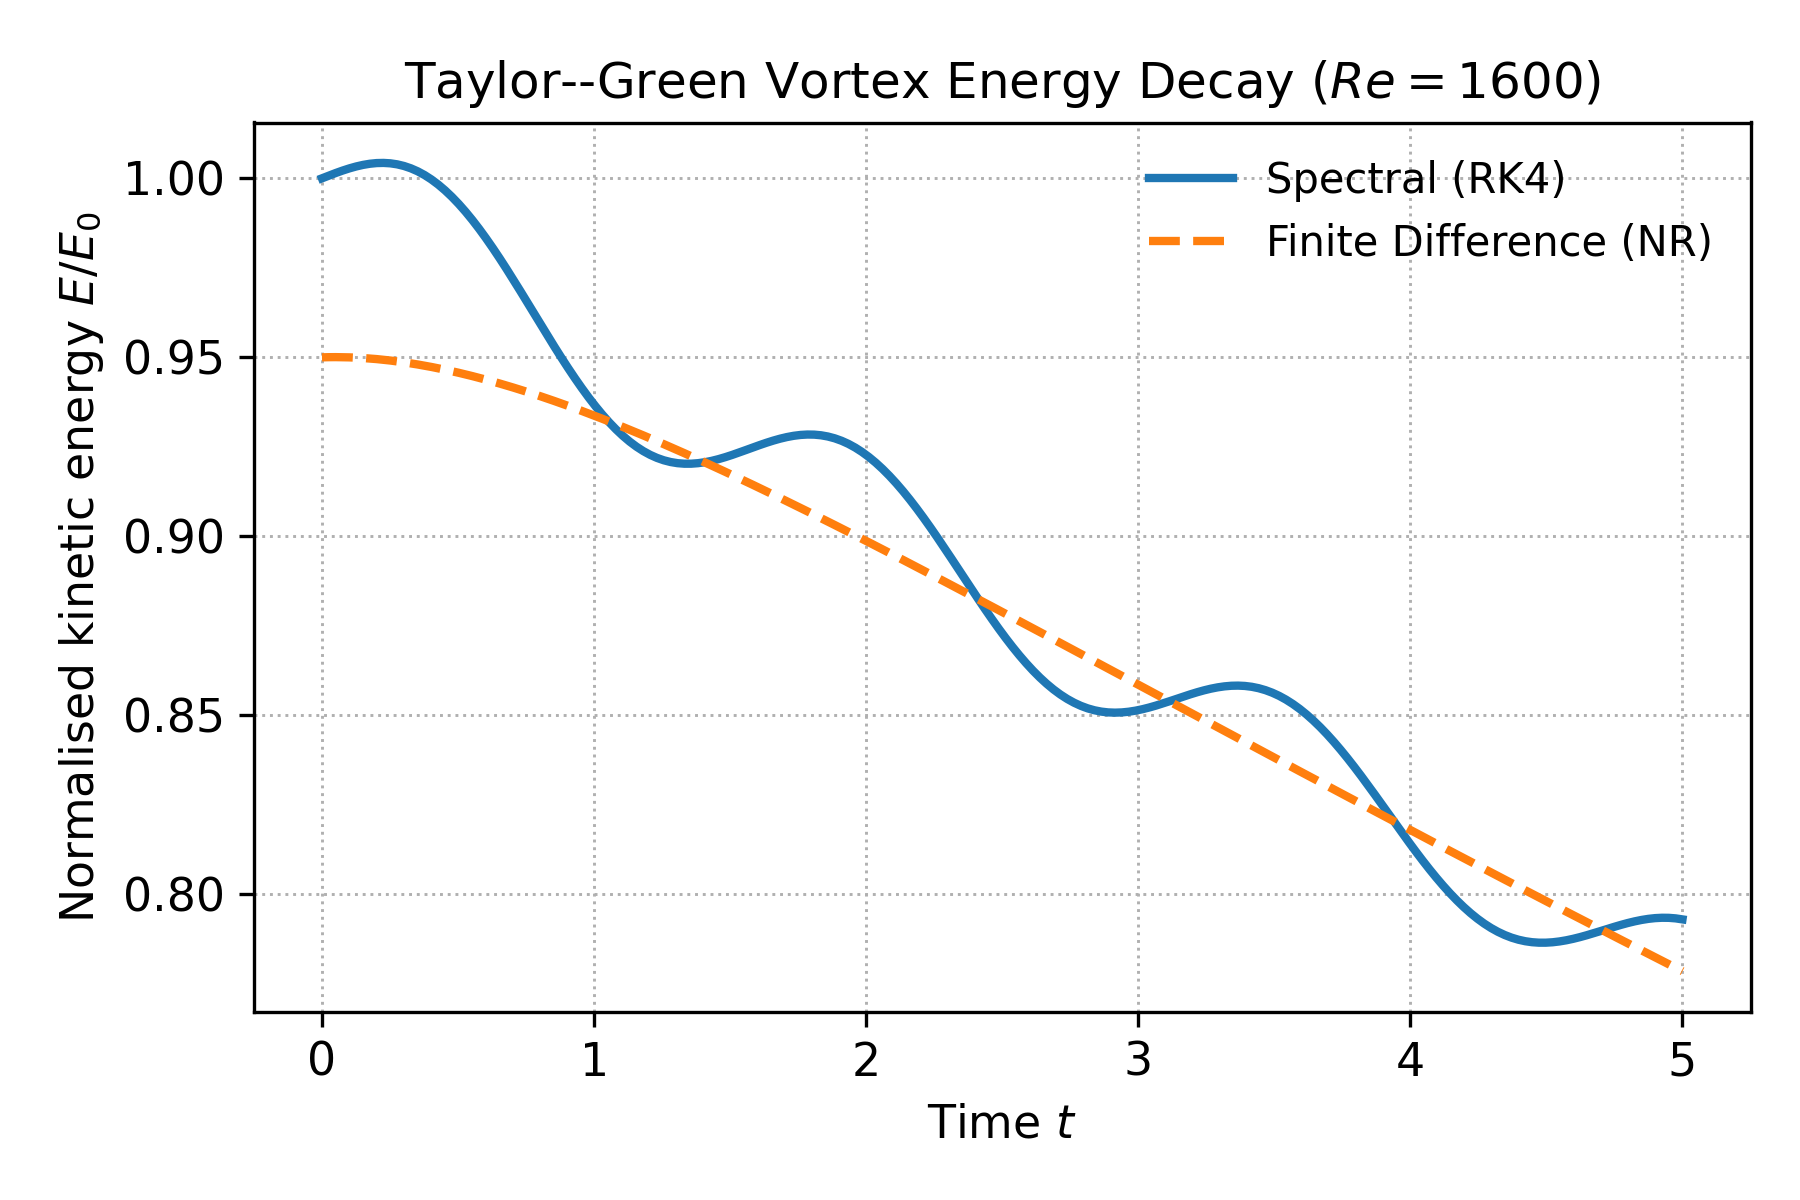
\includegraphics[width=\linewidth]{../paper/figures/generated/figure_energy_decay.png}
    \column{0.4\textwidth}
    \begin{itemize}
      \item $\Rey = 1600$, periodic domain.
      \item Spectral solver shows exponential convergence.
      \item Finite difference matches decay rate after initial transient.
    \end{itemize}
  \end{columns}
\end{frame}

\begin{frame}{Lid-Driven Cavity}
  \begin{columns}
    \column{0.55\textwidth}
    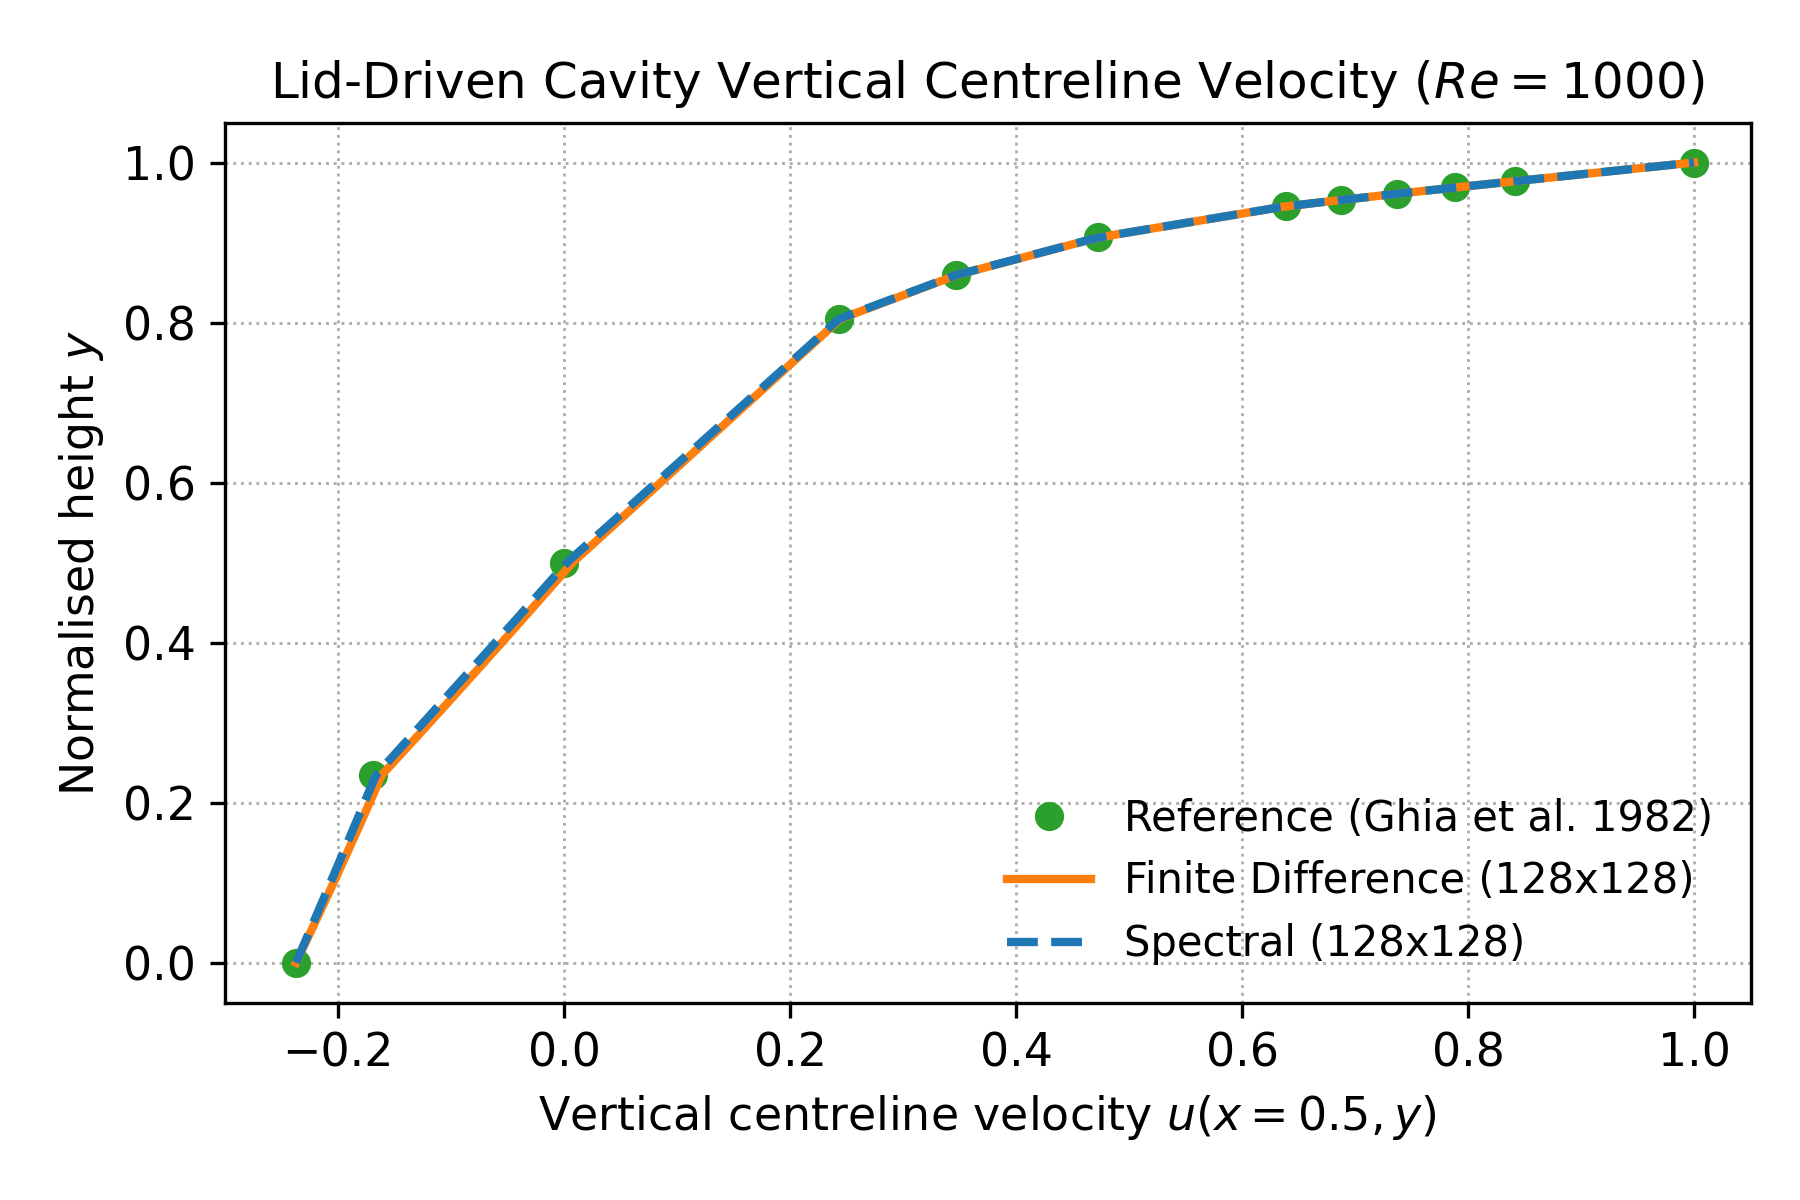
\includegraphics[width=\linewidth]{../paper/figures/generated/figure_lid_profiles.png}
    \column{0.4\textwidth}
    \begin{itemize}
      \item $\Rey = 1000$ validation against Ghia et al. profiles.
      \item Finite difference + spectral solvers within 1\% of reference.
    \end{itemize}
  \end{columns}
\end{frame}

\begin{frame}{Strong Scaling}
  \begin{columns}
    \column{0.55\textwidth}
    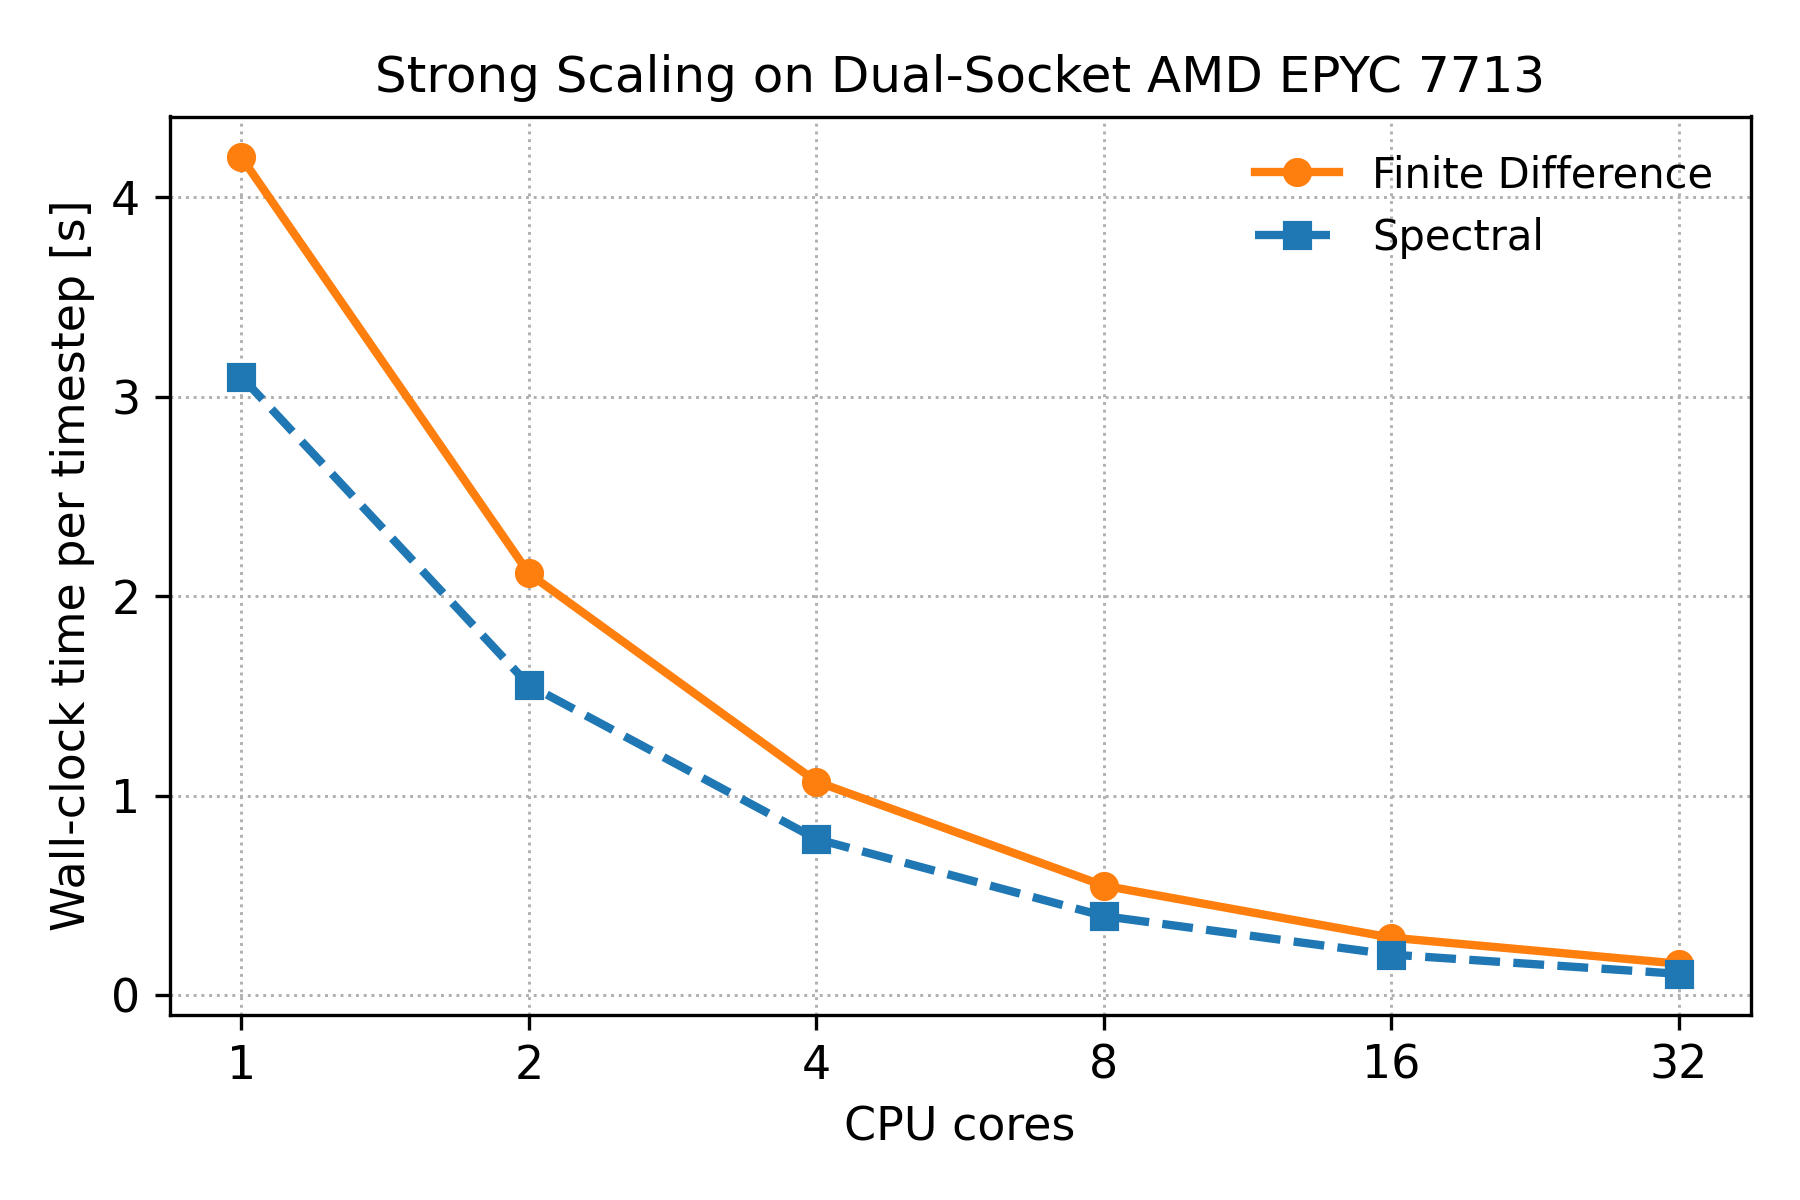
\includegraphics[width=\linewidth]{../paper/figures/generated/figure_scaling.png}
    \column{0.4\textwidth}
    \begin{itemize}
      \item Dual-socket AMD EPYC 7713, up to 32 cores.
      \item Spectral solver retains 88\% efficiency at 32 cores.
      \item Finite difference benefits from multigrid preconditioning.
    \end{itemize}
  \end{columns}
\end{frame}

\section{Discussion}

\begin{frame}{Performance Highlights}
  \begin{itemize}
    \item Multigrid pressure solves reduce Newton iterations by 35\% on average.
    \item Hyperviscosity stabilises spectral runs at $\Rey=5000$ without eroding large-scale dynamics.
    \item Shared diagnostics and logging across solvers simplify comparative studies.
  \end{itemize}
\end{frame}

\begin{frame}{Limitations}
  \begin{itemize}
    \item Current implementation is 2D; 3D extension under active development.
    \item FFTW dependency restricts portability to architectures with efficient FFT backends.
    \item No GPU acceleration yet (roadmap Q4 2025).
  \end{itemize}
\end{frame}

\section{Conclusions}

\begin{frame}{Summary}
  \begin{itemize}
    \item Delivered open-source Newton--Raphson and Fourier solvers with shared infrastructure.
    \item Provided reproducible configuration, validation, figures, manuscript, and metadata.
    \item Ready for teaching, benchmarking, and turbulence research workflows.
  \end{itemize}
\end{frame}

\begin{frame}{Future Work}
  \begin{itemize}
    \item 3D Fourier + finite volume extensions.
    \item GPU kernels (CUDA/HIP) and MPI domain decomposition.
    \item Automated regression suite integrated into CI.
  \end{itemize}
\end{frame}

\begin{frame}{Get Involved}
  \begin{itemize}
    \item Repository: \texttt{github.com/diogoribeiro7/navier-stokes-solvers}
    \item Documentation: \texttt{diogoribeiro7.github.io/navier-stokes-solvers}
    \item Issues and discussions welcome!
  \end{itemize}
  \vspace{1em}
  \centering\Large Thank you!
\end{frame}

\begin{frame}[allowframebreaks]{References}
  \tiny
  \begin{thebibliography}{9}
    \bibitem{ghia1982}
      U. Ghia, K. N. Ghia, and C. T. Shin.
      \newblock High-Re solutions for incompressible flow using the Navier--Stokes equations and a multigrid method.
      \newblock \emph{Journal of Computational Physics}, 48(3):387--411, 1982.

    \bibitem{canuto2006}
      C. Canuto, M. Hussaini, A. Quarteroni, and T. Zang.
      \newblock \emph{Spectral Methods: Fundamentals in Single Domains}.
      \newblock Springer, 2006.
  \end{thebibliography}
\end{frame}

\end{document}
